\documentclass[conference]{IEEEtran}
\usepackage[T1]{fontenc}
\usepackage{lmodern}
\usepackage{graphicx}
\graphicspath{{img/}{tp2/docs/img/}}
\usepackage{booktabs}
\usepackage{amsmath}
\usepackage{amssymb}
\usepackage{float}
\usepackage{hyperref}
\usepackage{tikz}
\usetikzlibrary{arrows.meta,positioning}
\setlength{\emergencystretch}{1.5em}

\title{OS202 -- TD2: Ford Fulkerson}
\author{Santiago Florido Gomez}

\begin{document}
\maketitle

\begin{abstract}
This report presents Ford--Fulkerson applications on flow networks, including maximum-flow
computations, minimum cuts, and unit-capacity models for matching and disjoint-path problems.
\end{abstract}

\section{Introduction}
In the present document, we will present applications of flow network modeling aimed at optimizing the circulation of resources in systems with limited capacities, mainly by applying the Ford--Fulkerson algorithm. With this objective, we seek to find maximum flows (i.e., the maximum throughput), detect bottlenecks, and enable assignment and matching in resource-allocation problems, such as the lock-and-key problem for opening a safe. Finally, we consider the use of Ford--Fulkerson on graphs with unit capacities in order to find disjoint routes in systems that require redundancy and robustness.

\section{Ford--Fulkerson}
\begin{figure}[H]
\centering
\includegraphics[width=\columnwidth]{img/ford_fulk1.png}
\caption{Flow network for Ford--Fulkerson (arc labels are capacities).}
\label{fig:ford-fulkerson-network}
\end{figure}
\textbf{Capacities}
\begin{align*}
&s\to a:8,\quad s\to c:4,\quad s\to e:6,\\
&a\to b:10,\quad a\to d:4,\\
&c\to d:1,\\
&e\to t:2,\\
&d\to t:6,\\
&b\to t:8.
\end{align*}

\textbf{Augmenting paths using ontly paths in alphabetical order}
\begin{enumerate}
\item $P_1: s\to a\to b\to t,\quad \Delta_1=\min(8,10,8)=8$
\item $P_2: s\to c\to d\to t,\quad \Delta_2=\min(4,1,6)=1$
\item $P_3: s\to e\to t,\quad \Delta_3=\min(6,2)=2$
\end{enumerate}

\textbf{Final flow (nonzero arcs)}
\begin{align*}
&f(s,a)=8,\quad f(a,b)=8,\quad f(b,t)=8,\\
&f(s,c)=1,\quad f(c,d)=1,\quad f(d,t)=1,\\
&f(s,e)=2,\quad f(e,t)=2.
\end{align*}

\[
|f| = 11.
\]
By applying the Ford--Fulkerson algorithm, the maximum flows that can be obtained while taking the capacities into account are as follows:

\begin{itemize}
  \item \texttt{'s' - 'a' (8.0)}
  \item \texttt{'s' - 'c' (3.0)}
  \item \texttt{'s' - 'e' (4.0)}
  \item \texttt{'a' - 'b' (4.0)}
  \item \texttt{'a' - 'd' (4.0)}
  \item \texttt{'b' - 't' (8.0)}
  \item \texttt{'c' - 'b' (2.0)}
  \item \texttt{'c' - 'd' (1.0)}
  \item \texttt{'d' - 't' (5.0)}
  \item \texttt{'e' - 'b' (2.0)}
  \item \texttt{'e' - 't' (2.0)}
\end{itemize}

To identify an appropriate way to improve the system's minimum flow, it is useful to analyze the minimum cuts resulting from applying Ford--Fulkerson, which are:
\[
S^*=\{s,a,b,c,e\},\qquad T^*=\{d,t\}.
\]
Given these minimum cuts, it becomes clear that it is advisable to increase the capacity of the arcs that go from \(S^*\) to \(T^*\), since those arcs act as bottlenecks that restrict the flow.

\begin{figure}[H]
\centering
\includegraphics[width=\columnwidth]{img/ford_fulk2.png}
\caption{Additional Ford--Fulkerson examples (arc labels are capacities).}
\label{fig:ford-fulkerson-examples}
\end{figure}

The Ford--Fulkerson algorithm was applied to the two networks shown in Figure~\ref{fig:ford-fulkerson-examples}. The resulting maximum flows and minimum cuts are:

\textbf{Graph 1 (left network).} Maximum flow value: $\lvert f \rvert = 23$. Nonzero flow arcs:
\begin{itemize}
  \item \texttt{'s' - '1' (12.0)}
  \item \texttt{'s' - '2' (11.0)}
  \item \texttt{'1' - '3' (12.0)}
  \item \texttt{'2' - '4' (11.0)}
  \item \texttt{'3' - 't' (19.0)}
  \item \texttt{'4' - '3' (7.0)}
  \item \texttt{'4' - 't' (4.0)}
\end{itemize}
Minimum cut: $S^*=\{s,1,2,4\}$, $T^*=\{3,t\}$.

\textbf{Graph 2 (right network).} Maximum flow value: $\lvert f \rvert = 30$. Nonzero flow arcs:
\begin{itemize}
  \item \texttt{'s' - 'A' (10.0)}
  \item \texttt{'s' - 'C' (10.0)}
  \item \texttt{'s' - 'E' (10.0)}
  \item \texttt{'A' - 'B' (8.0)}
  \item \texttt{'A' - 'D' (2.0)}
  \item \texttt{'C' - 'B' (2.0)}
  \item \texttt{'C' - 'D' (8.0)}
  \item \texttt{'E' - 'F' (10.0)}
  \item \texttt{'B' - 't' (10.0)}
  \item \texttt{'D' - 't' (10.0)}
  \item \texttt{'F' - 't' (10.0)}
\end{itemize}
Minimum cut: $S^*=\{s,C,E,F\}$, $T^*=\{A,B,D,t\}$.

I would propose solving the problem as follows: define a source node \(s\) from which arcs of capacity \(1\) go to each key that can be used, since each key can only be used once. Then, each key is connected by arcs of capacity \(1\) to the drawers it can open. Finally, from those drawers, define edges of capacity \(1\) to the sink \(t\). I would implement a Ford--Fulkerson algorithm in order to identify the maximum flow, i.e., the maximum number of drawers that can be opened simultaneously given the available keys.

\begin{figure}[h]
\centering
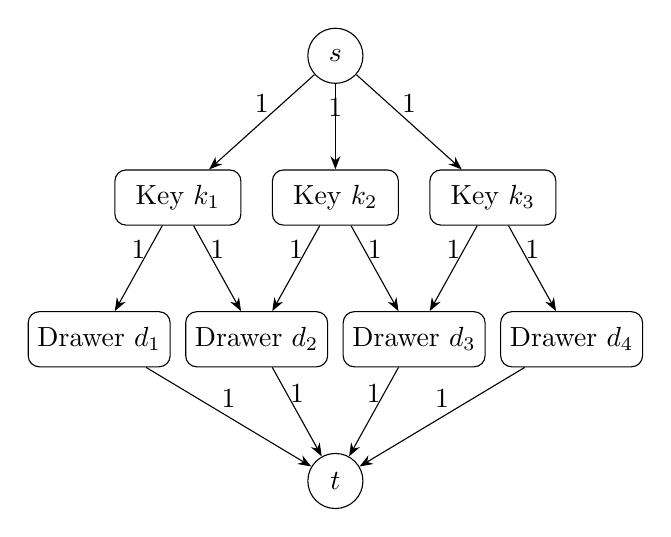
\begin{tikzpicture}[
  >=Stealth,
  node distance=10mm and 18mm,
  key/.style={draw, rounded corners, minimum width=16mm, minimum height=7mm},
  drawer/.style={draw, rounded corners, minimum width=18mm, minimum height=7mm},
  term/.style={draw, circle, minimum size=7mm}
]

% Nodes (vertical layout)
\node[term] (s) at (0, 0) {$s$};

\node[key] (k1) at (-2, -1.8) {Key $k_1$};
\node[key] (k2) at (0,  -1.8) {Key $k_2$};
\node[key] (k3) at (2,  -1.8) {Key $k_3$};

\node[drawer] (d1) at (-3, -3.6) {Drawer $d_1$};
\node[drawer] (d2) at (-1, -3.6) {Drawer $d_2$};
\node[drawer] (d3) at (1,  -3.6) {Drawer $d_3$};
\node[drawer] (d4) at (3,  -3.6) {Drawer $d_4$};

\node[term] (t) at (0, -5.4) {$t$};

% Arcs: source -> keys (capacity 1)
\draw[->] (s) -- (k1) node[midway, above] {$1$};
\draw[->] (s) -- (k2) node[midway, above] {$1$};
\draw[->] (s) -- (k3) node[midway, above] {$1$};

% Arcs: keys -> drawers (capacity 1)  %%% EDIT THESE CONNECTIONS AS NEEDED %%%
\draw[->] (k1) -- (d1) node[midway, above] {$1$};
\draw[->] (k1) -- (d2) node[midway, above] {$1$};

\draw[->] (k2) -- (d2) node[midway, above] {$1$};
\draw[->] (k2) -- (d3) node[midway, above] {$1$};

\draw[->] (k3) -- (d3) node[midway, above] {$1$};
\draw[->] (k3) -- (d4) node[midway, above] {$1$};

% Arcs: drawers -> sink (capacity 1)
\draw[->] (d1) -- (t) node[midway, above] {$1$};
\draw[->] (d2) -- (t) node[midway, above] {$1$};
\draw[->] (d3) -- (t) node[midway, above] {$1$};
\draw[->] (d4) -- (t) node[midway, above] {$1$};

\end{tikzpicture}
\caption{Flow network model: each key can be used at most once, and each opened drawer contributes one unit of flow.}
\end{figure}

\begin{figure}[H]
\centering
\includegraphics[width=\columnwidth]{img/disjoint_paths.png}
\caption{Graph used for the disjoint paths problem.}
\label{fig:disjoint-paths}
\end{figure}

The \emph{disjoint paths} problem is addressed analogously to the keys-and-drawers formulation: it is transformed into a \textbf{maximum flow} problem and solved with \textbf{Ford--Fulkerson} using \textbf{unit capacities}. These capacities ensure that the resulting paths are \textbf{unique} and \textbf{disjoint} according to the chosen criterion.

There are two main levels of separation:

\begin{itemize}
  \item \textbf{Arc-disjoint:} assign capacity $1$ to every arc. This prevents any additional unit of flow from reusing a saturated arc, so the set of paths induced by the maximum flow is edge-disjoint.

  \item \textbf{Vertex-disjoint:} in addition to unit capacities, forbid two paths from sharing an intermediate vertex. This is done via \emph{node splitting}: each vertex $v$ is replaced by two subnodes $v_{\text{in}}$ and $v_{\text{out}}$, connected by an arc $(v_{\text{in}},v_{\text{out}})$ of capacity $1$. Then, all incoming edges to $v$ are redirected to $v_{\text{in}}$ and all outgoing edges leave from $v_{\text{out}}$. This enforces a unit capacity per vertex.
\end{itemize}

Therefore, to solve the instance in Figure~\ref{fig:disjoint-paths}, both strategies must be implemented: the first to obtain arc-disjoint paths, and the second (with node splitting) to obtain vertex-disjoint paths.

The Ford--Fulkerson results for the graph in Figure~\ref{fig:disjoint-paths} are:

\textbf{Arc-disjoint (unit capacities on arcs).} Maximum flow value: $\lvert f \rvert = 3$. Nonzero flow arcs:
\begin{itemize}
  \item \texttt{'s' - 'a' (1.0)}
  \item \texttt{'s' - 'g' (1.0)}
  \item \texttt{'s' - 'e' (1.0)}
  \item \texttt{'a' - 'b' (1.0)}
  \item \texttt{'g' - 'c' (1.0)}
  \item \texttt{'e' - 'h' (1.0)}
  \item \texttt{'b' - 'd' (1.0)}
  \item \texttt{'c' - 'f' (1.0)}
  \item \texttt{'h' - 't' (1.0)}
  \item \texttt{'f' - 't' (1.0)}
  \item \texttt{'d' - 't' (1.0)}
\end{itemize}

\textbf{Vertex-disjoint (node splitting with unit capacities).} Maximum flow value: $\lvert f \rvert = 3$. Nonzero flow arcs:
\begin{itemize}
  \item \texttt{'s' - 'a\_in' (1.0)}
  \item \texttt{'s' - 'g\_in' (1.0)}
  \item \texttt{'s' - 'e\_in' (1.0)}
  \item \texttt{'a\_in' - 'a\_out' (1.0)}
  \item \texttt{'a\_out' - 'b\_in' (1.0)}
  \item \texttt{'g\_in' - 'g\_out' (1.0)}
  \item \texttt{'g\_out' - 'c\_in' (1.0)}
  \item \texttt{'e\_in' - 'e\_out' (1.0)}
  \item \texttt{'e\_out' - 'h\_in' (1.0)}
  \item \texttt{'b\_in' - 'b\_out' (1.0)}
  \item \texttt{'b\_out' - 'd\_in' (1.0)}
  \item \texttt{'c\_in' - 'c\_out' (1.0)}
  \item \texttt{'c\_out' - 'f\_in' (1.0)}
  \item \texttt{'h\_in' - 'h\_out' (1.0)}
  \item \texttt{'h\_out' - 't' (1.0)}
  \item \texttt{'f\_in' - 'f\_out' (1.0)}
  \item \texttt{'f\_out' - 't' (1.0)}
  \item \texttt{'d\_in' - 'd\_out' (1.0)}
  \item \texttt{'d\_out' - 't' (1.0)}
\end{itemize}

\end{document}
